\subsection{JavaScript - Basics}
\subsubsection{Incorporare JS in HTML}
\begin{lstlisting}[language=html]
<!DOCTYPE html>
<html>
    <body>
    <h1>My Web Page</h1>
    <p id="demo">A Paragraph</p>
    <button type="button" onclick="myFunction()">Try it</button>
    <script>
        function myFunction() {
        document.getElementById("demo").innerHTML = "Paragraph changed.";
        }
    </script>
    </body>
</html>
\end{lstlisting}
Solitamente si preferisce includere il documento JS a parte e poi importarlo con delle chiamate nel documento HTML.

\subsubsection{Parole riservate per JavaScript}
\begin{figure}[h!]
    \centering
    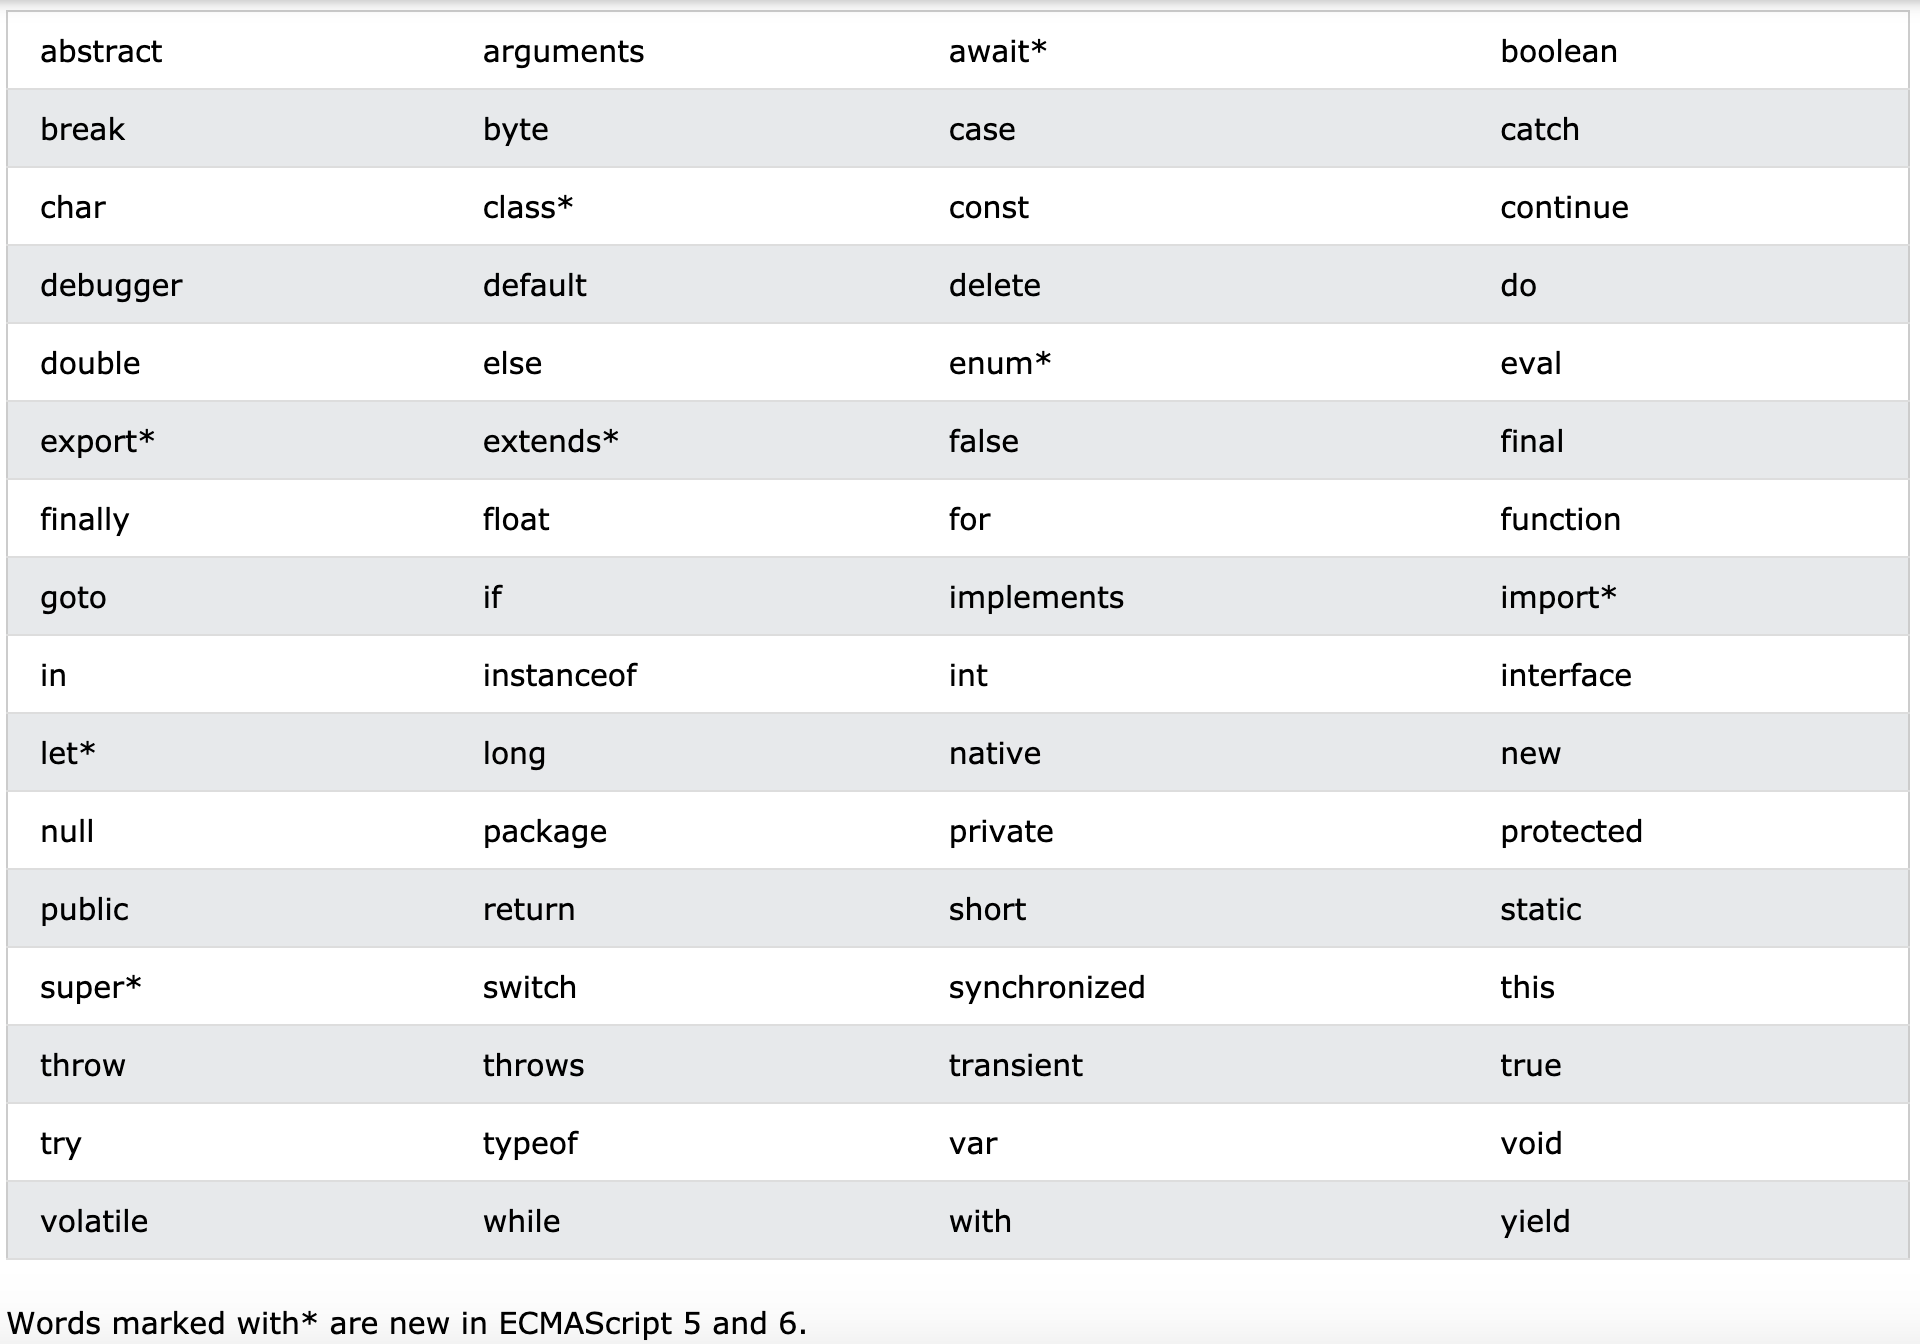
\includegraphics[width=0.8\linewidth]{imgs/4 - reserved keyword.png}
    \label{fig:ReserverKeyword}
    \caption{Parole riservate in JS}
\end{figure}

\subsubsection{Costanti e variabili}
Si usa \textbf{const} per le costanti e \textbf{let} per le variabili.

\subsubsection{Funzioni}
\begin{lstlisting}
function myFunction(p1, p2) {
    return p1 * p2;
}
\end{lstlisting}
\subsubsection{ArrowFunction}
\begin{lstlisting}
    const sum = (x, y) => { return x + y; };
\end{lstlisting}
\subsubsection{Oggetti}
\begin{lstlisting}
let person = {
    firstName:"John",
    lastName:"Doe",
    age:50,
    eyeColor:"blue",
    fullName:function() {return this.firstName + " " + this.lastName;}
};
\end{lstlisting}
Si può accedere ad un oggetto in due modi:
\begin{itemize}
    \item objectName.propertyName
    \item objectName[propertyName]
\end{itemize}
Per accedere ai metodi: objectName.methodName()

